\documentclass[a4paper, 12pt]{letter}
\usepackage[utf8]{inputenc}
\usepackage[scaled]{helvet}
\renewcommand\familydefault{\sfdefault}
\usepackage[T1]{fontenc}
\usepackage[francais]{babel}
\usepackage[left=2.5cm,top=6cm,right=2.5cm,bottom=2.5cm]{geometry}
\usepackage{graphicx}
\begin{document}
\pagenumbering{gobble} %no page number

% ---------------- Le contenu commence ici ----------------
\hbox to \textwidth{\hfill
	\vbox{
		\hbox{<title>}
		\hbox{<firstName> <lastName>}
		\hbox{<livesAt>}
		\hbox{<street> <numStreet>}
		\hbox{<postCode> <locality>}
		\bigbreak
		\bigbreak
		\bigbreak
		\hbox{Veyrier, le <sendDate> / <initials>}
	}
}

\bigbreak

\begin{flushleft}
	\textbf{Réponse négative après mise en suspens}
	\line(1,0){455}
\end{flushleft}
\bigbreak

<title>,

Nous faisons suite à notre courrier du <requestDate> par lequel nous vous informions que votre candidature était conservée pour une durée de 6 mois.

Malheureusement, n’ayant eu aucun poste à vous proposer durant cette période, nous nous permettons de vous retourner votre dossier. 

Nous vous remercions de la confiance et de l’intérêt manifesté pour l’EMS Les Châtaigniers et vous souhaitons de trouver rapidement un emploi conforme à vos aspirations.

Veuillez agréer, <title>, nos sincères salutations.

\bigbreak
\bigbreak
\bigbreak
\bigbreak

\hbox to \textwidth{\hfill
	\vbox{
		\hbox{EMS Les Châtaigniers}
	}
}
\begin{flushright}
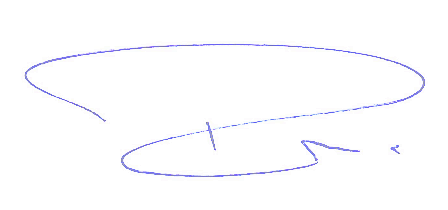
\includegraphics{sign.png}
\end{flushright}

\hbox to \textwidth{\hfill
	\vbox{
		\hbox{Samuel Moix, Directeur adjoint}
	}
}

\bigbreak
\bigbreak

<folder>

\end{document}
